% A second note beside the APP1 report, assessing a proposed representation and
% solver: the maze as a binary tree of branching points, walked by local moves.
% It stands alone and borrows only the shared preamble.
\documentclass[11pt,a4paper]{article}
% Everything the document needs before the first section: packages, page setup,
% the theorem and pseudocode environments, the drawing styles shared by every
% figure, and the notation macros. Sections and figures declare nothing of their
% own, so one edit here restyles the whole report.

\usepackage[T1]{fontenc}
\usepackage[utf8]{inputenc}
\usepackage{lmodern}
\usepackage[english]{babel}
\usepackage{microtype}
\usepackage{geometry}
\geometry{margin=2.4cm}

\usepackage{amsmath,amssymb,amsthm}
\usepackage{booktabs}
\usepackage{enumitem}
\usepackage{caption}
\usepackage{subcaption}
\usepackage{xcolor}
\usepackage[linesnumbered,ruled,vlined]{algorithm2e}
\usepackage{tikz}
\usetikzlibrary{arrows.meta,calc,fit,positioning,backgrounds}
\usepackage{import}
\usepackage{hyperref}
\usepackage{bookmark}

% --- Shared palette ------------------------------------------------------
% Named by the role each colour plays in a figure, not by the colour itself,
% so a change of palette does not turn every caption into a lie.
\definecolor{linkblue}{HTML}{1F4E79}
\definecolor{doorgreen}{HTML}{2E7D32}   % an edge kept: a door
\definecolor{wallred}{HTML}{C62828}     % an edge deleted: a wall segment
\definecolor{cellgrey}{HTML}{ECEFF1}    % the area a region covers
\definecolor{exitorange}{HTML}{E65100}  % the single exit cell

\hypersetup{colorlinks=true,linkcolor=linkblue,citecolor=linkblue,urlcolor=linkblue}

% --- Shared drawing styles ----------------------------------------------
\tikzset{
  cell/.style     = {draw=black!45, fill=cellgrey, minimum size=9mm},
  node vertex/.style = {circle, draw=black!70, fill=white, inner sep=0pt,
                        minimum size=4.2mm, font=\scriptsize},
  exit vertex/.style = {node vertex, draw=exitorange, very thick,
                        fill=exitorange!12},
  door/.style     = {doorgreen, line width=1.1pt},
  wall/.style     = {wallred, line width=1.1pt, dash pattern=on 2pt off 2pt},
  wall segment/.style = {wallred, line width=1.6pt},
  region/.style   = {draw=black!60, fill=cellgrey, thick},
  link/.style     = {-{Stealth[length=2mm]}, black!65},
  tree node/.style = {draw=black!70, rounded corners=1.5pt, inner sep=2.5pt,
                      font=\scriptsize, fill=white},
  tree leaf/.style = {tree node, draw=doorgreen!80!black, fill=doorgreen!8},
  tree edge/.style = {black!55},
}

% --- Theorem-like environments ------------------------------------------
\theoremstyle{definition}
\newtheorem{definition}{Definition}
\theoremstyle{plain}
\newtheorem{proposition}{Proposition}
\theoremstyle{remark}
\newtheorem*{remark}{Remark}

% --- Notation ------------------------------------------------------------
% The report says "the grid graph" and "the maze" constantly; these keep the
% symbols identical in prose, in displays and in pseudocode.
\newcommand{\gridgraph}{G_{\text{grid}}}
\newcommand{\gridedges}{E_{\text{grid}}}
\newcommand{\maze}{M}
\newcommand{\cells}{V}
\newcommand{\region}[2]{[#1]\times[#2]}
\newcommand{\exitcell}{v_{\text{exit}}}
\SetKwProg{Fn}{Function}{:}{}


\title{The maze as a tree of branching points\\
       \large walking it by local moves --- a note beside the APP1 report}
\author{Mohamed Ali Tewfik Hamlil\\[2pt]
  \small M1 Artificial Intelligence, Universit\'e Grenoble Alpes}
\date{\today}

\begin{document}
\maketitle

\begin{abstract}
A proposal: store the maze not as a set of cells but as a binary tree whose
nodes hold branching points, give every cell an address in that tree, and solve
by walking from the start's node to the exit's, each step moving to whichever of
the parent, the children and the sibling lies nearest the exit. This note takes
it apart. The \emph{structure} is right and is the one the generator already
builds. The \emph{navigation rule} is not: it is greedy best-first search, which
is neither optimal nor complete, and on $200$ mazes of $32\times32$ it stopped
at a local minimum $199$ times. Replacing ``nearest the exit'' by ``which side
holds the exit's address'' makes the same walk optimal and $\Theta(\log n)$ ---
measured at $1.06\log_2 n$ moves. What that buys, and what it does not, is set
out at the end.
\end{abstract}

\section{The proposal, stated}

\begin{description}[leftmargin=*,style=nextline,itemsep=5pt]
  \item[Structure.] A binary tree instead of a set of cells. Each internal node
    stores the \keyterm{branching point} of the division that created it --- the
    cell its single door sits on. Each leaf is a region. A cell's
    \keyterm{address} is the sequence of turns from the root to its leaf.
  \item[Solver.] The start and the exit are given as addresses. From the start's
    node, each step moves to whichever of the \keyterm{parent}, the
    \keyterm{children} and the \keyterm{sibling} has its stored point nearest
    the exit, and stops on arrival.
\end{description}

Figure~\ref{fig:addresses} is the structure. It is worth saying at once that
this is not a new structure: it is the region tree the generator of the report
already returns, with the door recorded at each node.

% The structure under discussion: a binary tree whose internal nodes hold the
% branching point of the division that made them, and whose leaves are cells.
% A cell's address is the sequence of turns that reaches its leaf.
\begin{figure}[htbp]
  \centering
  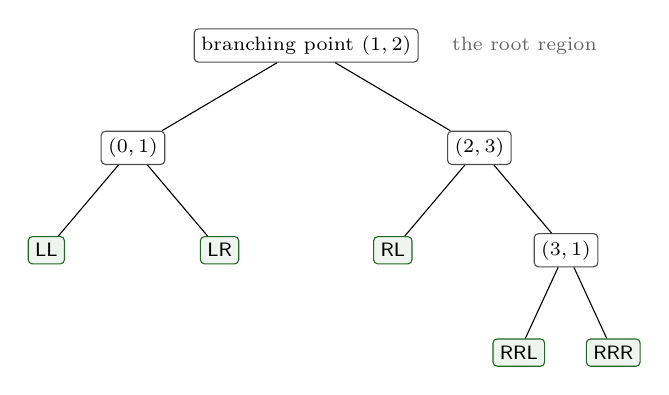
\begin{tikzpicture}[scale=1.0, level distance=13mm,
    level 1/.style={sibling distance=44mm},
    level 2/.style={sibling distance=22mm},
    level 3/.style={sibling distance=12mm}]
    \node[tree node] (root) {branching point $(1,2)$}
      child {node[tree node] {$(0,1)$}
        child {node[tree leaf] {\textsf{LL}}}
        child {node[tree leaf] {\textsf{LR}}}
      }
      child {node[tree node] {$(2,3)$}
        child {node[tree leaf] {\textsf{RL}}}
        child {node[tree node] {$(3,1)$}
          child {node[tree leaf] {\textsf{RRL}}}
          child {node[tree leaf] {\textsf{RRR}}}
        }
      };
    \node[font=\scriptsize, black!60, right=3mm of root] {the root region};
  \end{tikzpicture}
  \caption{The proposed structure. Each internal node stores the branching point
  of the division that created it --- the cell its single door sits on --- and
  each leaf is a region of the maze. A cell's \keyterm{address} is the sequence
  of turns from the root to its leaf, so \textsf{RRL} names one region in three
  characters. Sibling leaves are the two halves a single division separated, and
  are joined in the maze by that division's door alone.}
  \label{fig:addresses}
\end{figure}


The sibling move deserves a note of its own. A node's sibling is its parent's
other child, so a sibling move is a parent move followed by a child move --- a
shortcut, not new reach. It matters anyway, because in the maze two sibling
regions are joined by exactly one door, their parent's. \keyterm{A sibling move
is the only one of the three that corresponds to walking through a door.}

\section{Is it optimal? No, and it is not even complete}

\begin{keypoint}
The rule is \keyterm{greedy best-first search}: it ranks moves by an estimate of
the remaining distance and ignores the distance already travelled. Greedy
best-first is not optimal, and without a closed list it is not complete.
\end{keypoint}

Measured on $200$ mazes per size, start at one corner, exit at the other.

\begin{center}
\begin{tabular}{@{}llrrr@{}}
  \toprule
  Size & Variant & Reached the exit & Never terminated & Stuck \\
  \midrule
  $16\times16$ & as proposed        & $13$ & $187$ & --- \\
  $16\times16$ & with a visited set & $24$ & ---   & $176$ \\
  $32\times32$ & as proposed        & $6$  & $194$ & --- \\
  $32\times32$ & with a visited set & $7$  & ---   & $193$ \\
  $64\times64$ & as proposed        & $2$  & $198$ & --- \\
  $64\times64$ & with a visited set & $3$  & ---   & $197$ \\
  \bottomrule
\end{tabular}
\end{center}

At $64\times64$ the walk arrives \emph{once in a hundred}. Adding a visited set
converts non-termination into an honest failure, which is an improvement in
diagnosis and none at all in outcome.

\subsection{The failure mode, diagnosed}

Instrumenting the $32\times32$ runs separates two possible causes and finds only
one of them.

\begin{center}
\begin{tabular}{@{}lr@{}}
  \toprule
  Cause & Runs \\
  \midrule
  Stuck at a local minimum: no available move is nearer the exit & $199$ \\
  Cycled: revisited a node already seen & $0$ \\
  \bottomrule
\end{tabular}
\end{center}

So it is not oscillation. It is hill-climbing meeting a hill
(Figure~\ref{fig:local-minimum}).

% Why the greedy rule stops: the current node is nearer the exit than its
% parent, its two children and its sibling, and is not the goal.
\begin{figure}[htbp]
  \centering
  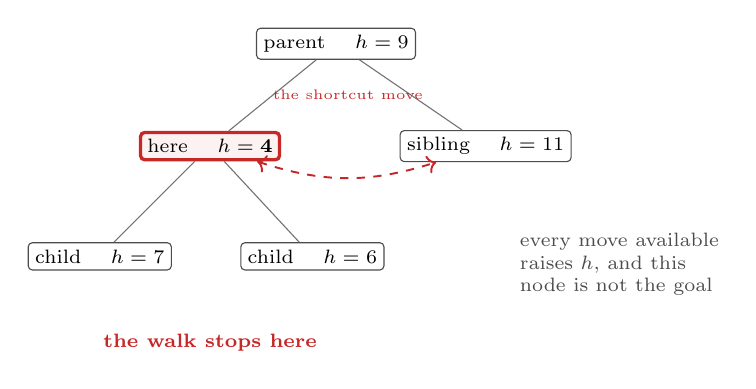
\begin{tikzpicture}[scale=1.0, every node/.style={font=\scriptsize}]
    \node[tree node] (parent) at (0,2.2) {parent \quad $h=9$};
    \node[tree node, draw=wallred, very thick, fill=wallred!6]
      (here) at (-1.6,0.9) {here \quad $h=\mathbf{4}$};
    \node[tree node] (sib) at (1.9,0.9) {sibling \quad $h=11$};
    \node[tree node] (l) at (-3.0,-0.5) {child \quad $h=7$};
    \node[tree node] (r) at (-0.3,-0.5) {child \quad $h=6$};
    \draw[tree edge] (parent) -- (here);
    \draw[tree edge] (parent) -- (sib);
    \draw[tree edge] (here) -- (l);
    \draw[tree edge] (here) -- (r);
    \draw[wallred, <->, dashed, line width=0.7pt] (here) to[bend right=18] (sib);
    \node[wallred, font=\tiny] at (0.15,1.55) {the shortcut move};
    \node[align=left, font=\scriptsize, black!70] at (3.6,-0.6)
      {every move available\\raises $h$, and this\\node is not the goal};
    \node[wallred, font=\scriptsize\bfseries] at (-1.6,-1.6) {the walk stops here};
  \end{tikzpicture}
  \caption{A local minimum, which is where the greedy rule ends $199$ runs in
  $200$. The stored branching point of the current node happens to lie nearer
  the exit than those of its parent, its two children and its sibling; no move
  improves $h$, and the exit is elsewhere. Nothing about the maze is wrong ---
  the rule is simply hill-climbing on a landscape with hills in it.}
  \label{fig:local-minimum}
\end{figure}


\subsection{Why the landscape has hills}

Two reasons, and the second is the one specific to this structure.

\begin{description}[leftmargin=*,style=nextline,itemsep=5pt]
  \item[Greedy search discards $g$.] Ranking only by the estimate to the goal
    means a step that walks into a cul-de-sac is taken whenever the cul-de-sac
    points the right way. This is generic and is why greedy best-first is not
    used when optimality matters.
  \item[A node's stored point is not where the walker is.] An internal node
    stands for a \emph{region}, not a position; its branching point is one cell
    inside it, chosen by the generator for reasons unrelated to the exit. Moving
    to a parent does not move the walker at all --- the parent covers the same
    ground and more. Ranking parents, children and siblings by a single stored
    cell compares objects that are not comparable.
\end{description}

\begin{keypoint}
The estimate answers ``how far is this node's door from the exit''. The walk
needs ``which way is the exit from here''. Those are different questions, and
the tree can answer the second exactly.
\end{keypoint}

\section{Time complexity of the proposal}

As stated, with no memory: \keyterm{unbounded}. The walk has no termination
argument, and on the evidence above it usually does not terminate. A step cap is
the only thing that ends it.

With a visited set: it terminates, because the tree is finite and no node is
entered twice, so it performs at most $O(L)$ moves on a tree of $L$ leaves,
which is $O(n)$. That is a bound on \emph{giving up}, not on succeeding.

\begin{keypoint}
Both figures are worse than Dijkstra's $\Theta(n)$, which at least always
returns the right answer. A cheaper wrong answer is not a better algorithm.
\end{keypoint}

\section{The rule that works: navigate by address}

The structure was never the problem. Replace the ranking.

\begin{algorithm}[H]
\caption{From the start's leaf to the exit's, by address.}
\label{alg:address-walk}
\SetKwFunction{Walk}{WalkToExitLeaf}
\SetKwFunction{Holds}{Holds}
\KwIn{the leaf holding the start, and the exit cell.}
\KwOut{the leaf holding the exit.}
\BlankLine
\Fn{\Walk{$\textit{leaf}$, $\exitcell$}}{
  $R \leftarrow \textit{leaf}$\;
  \While{$R$ \textup{does not contain} $\exitcell$}{
    $R \leftarrow R.\textit{parent}$\tcp*{climb to the lowest common ancestor}
  }
  \While{$R$ \textup{is not a leaf}}{
    $R \leftarrow$ whichever child contains $\exitcell$
      \tcp*{descend by address}
  }
  \Return $R$\;
}
\end{algorithm}

No distance is consulted. Each test is a comparison of the exit's coordinates
against a rectangle, and the walk is forced at every step: up while the region
is too small to contain the exit, then down the one branch that does.

\begin{proposition}
Algorithm~\ref{alg:address-walk} reaches the exit's leaf, and does so in the
fewest parent/child moves possible.
\end{proposition}

\begin{proof}
Climbing terminates: the root contains every cell. The first node reached that
contains the exit is the lowest common ancestor of the two leaves, since every
node on the way up was too small and ancestors only grow. Descending is
deterministic --- exactly one child contains the exit --- and ends at its leaf.
The moves made are $\mathrm{depth}(\textit{start})-\mathrm{depth}(\mathrm{lca})$
up and $\mathrm{depth}(\exitcell)-\mathrm{depth}(\mathrm{lca})$ down, which is
the length of the unique path between the two leaves in the tree, and no walk
between them can be shorter.
\end{proof}

Measured over $200$ mazes per size, against the optimal tree path each time:

\begin{center}
\begin{tabular}{@{}rrrrl@{}}
  \toprule
  $n$ & Moves & $\log_2 n$ & Moves $/\log_2 n$ & Optimal every run? \\
  \midrule
  $256$   & $8.4$  & $8$  & $1.05$ & yes \\
  $1024$  & $10.5$ & $10$ & $1.05$ & yes \\
  $4096$  & $12.8$ & $12$ & $1.07$ & yes \\
  $16384$ & $14.9$ & $14$ & $1.06$ & yes \\
  $65536$ & $17.1$ & $16$ & $1.07$ & yes \\
  \bottomrule
\end{tabular}
\end{center}

\begin{keypoint}
$\Theta(\log n)$, at about $1.06\log_2 n$ moves, and optimal on every run of
every size. The greedy rule reached the exit $1\%$ of the time; the address rule
reaches it always, in a number of moves bounded by the depth of the tree.
\end{keypoint}

\section{What this actually gives, and what it does not}

One qualification matters, and it is easy to miss.

\begin{keypoint}
Algorithm~\ref{alg:address-walk} finds the \keyterm{leaf}, not the
\keyterm{route}. It locates the exit's region and, on the way, the lowest common
ancestor --- whose door is the first door the route crosses. It does not
enumerate the rest.
\end{keypoint}

The three costs separate cleanly, and only the first is logarithmic.

\begin{center}
\begin{tabular}{@{}lll@{}}
  \toprule
  Question & Cost & How \\
  \midrule
  Which region holds the exit? Which door first? & $\Theta(\log n)$
    & Algorithm~\ref{alg:address-walk} \\
  How many doors between start and exit? & $\Theta(n^{0.68})$
    & the recursive decomposition \\
  Which cells, in order? & $\Theta(d)$
    & the size of the answer itself \\
  \bottomrule
\end{tabular}
\end{center}

The middle row is the subject of the companion note; the exponent is measured,
and comes from a branching recurrence whose one parameter is the probability
that a division separates the two endpoints.

\section{Verdict}

\begin{description}[leftmargin=*,style=nextline,itemsep=5pt]
  \item[The structure: keep it.] A binary tree of branching points with
    addressed leaves is the right representation, and the generator already
    produces it at no extra cost. It is also what the subject's learning
    objectives ask to be used.
  \item[The navigation rule: replace it.] Ranking parent, children and sibling
    by distance to the exit is greedy best-first search on an estimate attached
    to the wrong object. It is not optimal, not complete, and succeeded on
    $1$--$12\%$ of runs.
  \item[What replaces it is simpler, not harder.] An address comparison, no
    arithmetic, no estimate, optimal by construction and $\Theta(\log n)$.
\end{description}

The instinct behind the proposal --- that the tree already knows where the exit
is, and the solver should ask it rather than search the cells --- is right, and
is what both these notes are about. It is only the question put to the tree that
needed changing.

\end{document}
